\documentclass[10pt]{book}
\usepackage{cdtBook}
\usepackage{cambios}
\usepackage{usecases}


%\newcommand{\proceso}{Gestión Integral de Residuos Sólidos Urbanos }
\defSistema{SIDAM}

\title{\Sistema \\\LARGE{sistema de rex \\{\bf Prototipo 1}}}
\subtitle{Análisis de Requerimientos}
%\author{}

%\date{martes 11 de mayo de 2010}

%%%%%%%%%%%%%%%%%%%%%%%%%%%%%%%%%%%%%%%%%%%%%%%%%%%%%%%%%%%%%%%%
\begin{document}
\ThisLRCornerWallPaper{0.5}{images/agua.png}
\maketitle\thispagestyle{empty}

\frontmatter
\tableofcontents

\mainmatter


%=========================================================
\chapter{Alcance del prototipo}

	En este capítulo se describe el alcance del prototipo a desarrollar. El alcance del sistema se ha definido como se muestra en la figura~\ref{fig:casosDeUsoCompleto} en donde cada módulo se describe a continuación.

\begin{figure}[htbp!]
	\begin{center}
		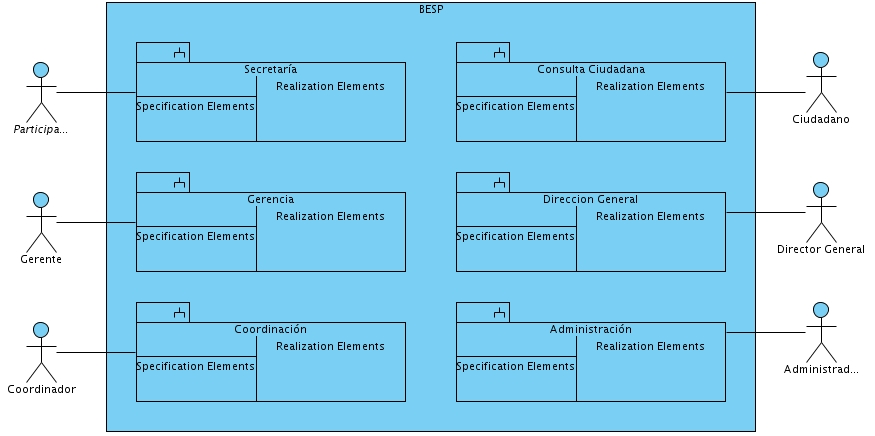
\includegraphics[width=1\textwidth]{images/alcance.jpg}
		\caption{Casos de uso del sistema.}
		\label{fig:casosDeUsoCompleto}
	\end{center}
\end{figure}

\begin{description}
	\item[Secretaría:] Incluye toda la funcionalidad para que la dirección pueda definir los Programas de la Secretaría y monitorearlos en un nivel muy general. El monitoreo incluye: avances, estado financiero global, semáforos y notas dirigidas a la gerencia. Así como la definición de Temas Transversales y Ejes temáticos.
	\item[Gerencia:] Incluye la funcionalidad para definir, actualizar y monitorear los programas y proyectos contemplados en cada Programa. Así como la definición de fechas y periodos para actualización de información por parte de los coordinadores.
	\item[Coordinación:] Incluye la definición de acciones, indicadores tanto físicos como financieros y metas para los proyectos asignados. Así como el reporte de avances de los proyectos y el registro de estudios derivados del proyecto.
	\item[Mensajes y Notificaciones:] Permite la comunicación en el sistema de los usuarios de una manera jerárquica por medio de mensajes simples.
	\item[Consulta Ciudadana:] Incluye el acceso a la información de los proyectos y los estudios realizados por parte del público en general.
	\item[Administración:] Administración de cuentas de usuarios y mantenimiento a los catálogos del sistema.
\end{description}

\section{Actores}

El sistema será usado por los usuarios cuyos perfiles se describen en la figura~\ref{fig:actores}.

\begin{figure}[htbp!]
	\begin{center}
		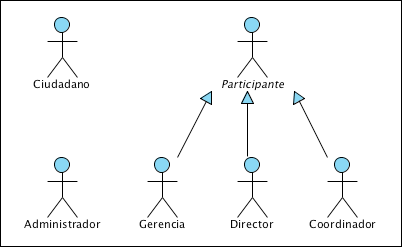
\includegraphics[width=.5\textwidth]{images/actores}
		\caption{Definición de actores del sistema.}
		\label{fig:actores}
	\end{center}
\end{figure}

%---------------------------------------------------------
\section{Alcance del prototipo}

%---------------------------------------------------------
\subsection{Cambios a la versión inicial}

	Los cambios a realizar sobre la Configuración inicial se resumen a continuación.

\begin{cambios}
	\PFCitem{PFC1 }{CU A1 Gestión de Usuarios}{\actualizar}
	\PFCitem{PFC2 }{CU A2 Gestión de Contactos}{\actualizar}
	\PFCitem{PFC2 }{CU A2.4 Gestión de Tipos de Contactos}{\actualizar}
	\PFCitem{PFC3 }{CU A3 Gestión de Tipo de Unidad}{\eliminar}
	\PFCitem{PFC4 }{CU A4 Gestión de Unidad}{\actualizar}
	\PFCitem{PFC5 }{CU A5 Gestión de Indicador}{\programar}
	\PFCitem{PFC6 }{CU A6 Gestión de Tipo de aviso}{\programar}
	\PFCitem{PFC7 }{CU A7 Gestión de Area}{\actualizar}
	\PFCitem{PFC8 }{CU A8 Gestión de Avisos}{\programar}
	\PFCitem{PFC9 }{CU A9 Gestión de Perfiles}{\eliminar}
	\PFCitem{PFC10}{CU A10 Gestión de Grupo}{\reemplazar{CU D Definir Estructura}}
	\PFCitem{PFC11}{CU A11 Gestión de Capitulo}{\reemplazar{CU A}}
\end{cambios}

Todos los cambios deben realizarse con base en las definiciones y consideraciones de este documento.

\subsection{Requerimientos que se agregan}

\subsection{Administración}
\begin{requerimientos}
	\FRitem{CU A12}{Gestión de proyectos Preregistrados}{Se consultan los proyectos preregistrados para su aprobación (con el registro del director responsable correspondiente) o su eliminación del sistema.}{}
\end{requerimientos}

\subsection{Gerencia}
\begin{requerimientos}
	\FRitem{CU G1}{Gestión de Programas}{Registro y actualización de los niveles y la estructura jerárquica del Programa de primer nivel.}{}
\end{requerimientos}

\subsection{Dirección}
\begin{requerimientos}
	\FRitem{CU D1}{Gestionar Programas de primer nivel}{Registro y actualización de información referente a los Programas de primer nivel y asignación de los directores correspondientes.}{}
	\FRitem{CU D2}{Gestión de Temas transversales}{Registro y actualización de los Temas transversales que aplican a todos los Programas de primer nivel.}{}
	\FRitem{CU D3}{Gestión de Ejes temáticos}{Registro y actualización de los Ejes temáticos que aplican a todos los Programas de primer nivel.}{}
\end{requerimientos}

\subsection{Coordinación}
\begin{requerimientos}
	\FRitem{CU C1}{Gestión de proyectos}{Consulta de proyectos registrados y preregistrados y preregistro de nuevos proyectos (esta ultima parte es con o sin cuenta de usuario).}{}
\end{requerimientos}

\subsection{Otro}
\begin{requerimientos}
	\FRitem{CU 0}{Control de acceso}{Inicio y cierre de sesión de todos los usuarios del sistema.}{}
\end{requerimientos}

%=========================================================
\chapter{Proceso de negocios}


%---------------------------------------------------------
\section{Proceso}

\begin{figure}[htbp!]
	\begin{center}
		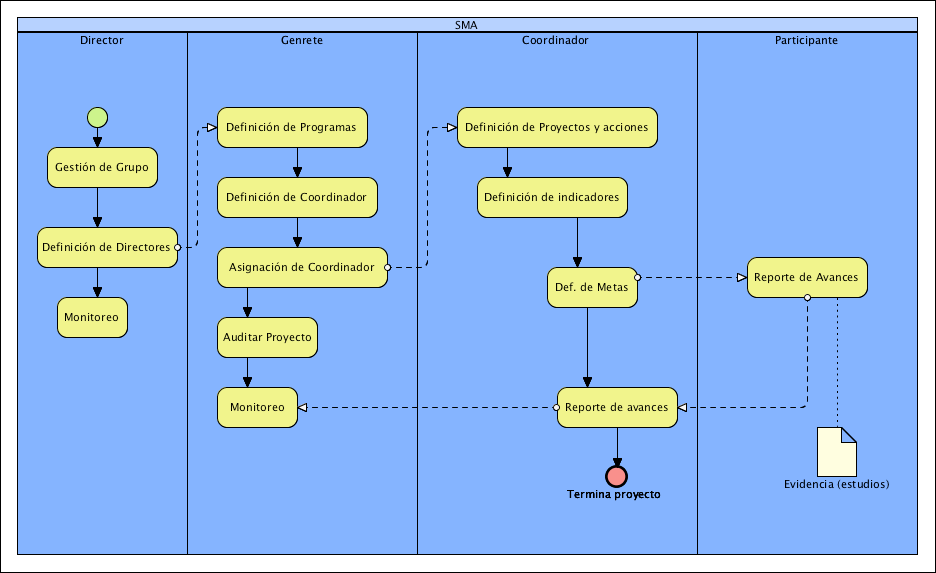
\includegraphics[width=.8\textwidth]{images/proceso}
		\caption{Proceso para el registro y definición de proyectos.}
		\label{fig:default}
	\end{center}
\end{figure}

%---------------------------------------------------------
\section{Reglas de Negocio}

\Instrucciones{Reglas de negocio: definición, hecho, afirmacion sobre un echo, restriccion, cálculo.}
\cfinput{reglas}


%=========================================================
\chapter{Modelo del comportamiento}

%---------------------------------------------------------
\section{Diagrama de CU}

\begin{figure}[htbp!]
	\begin{center}
		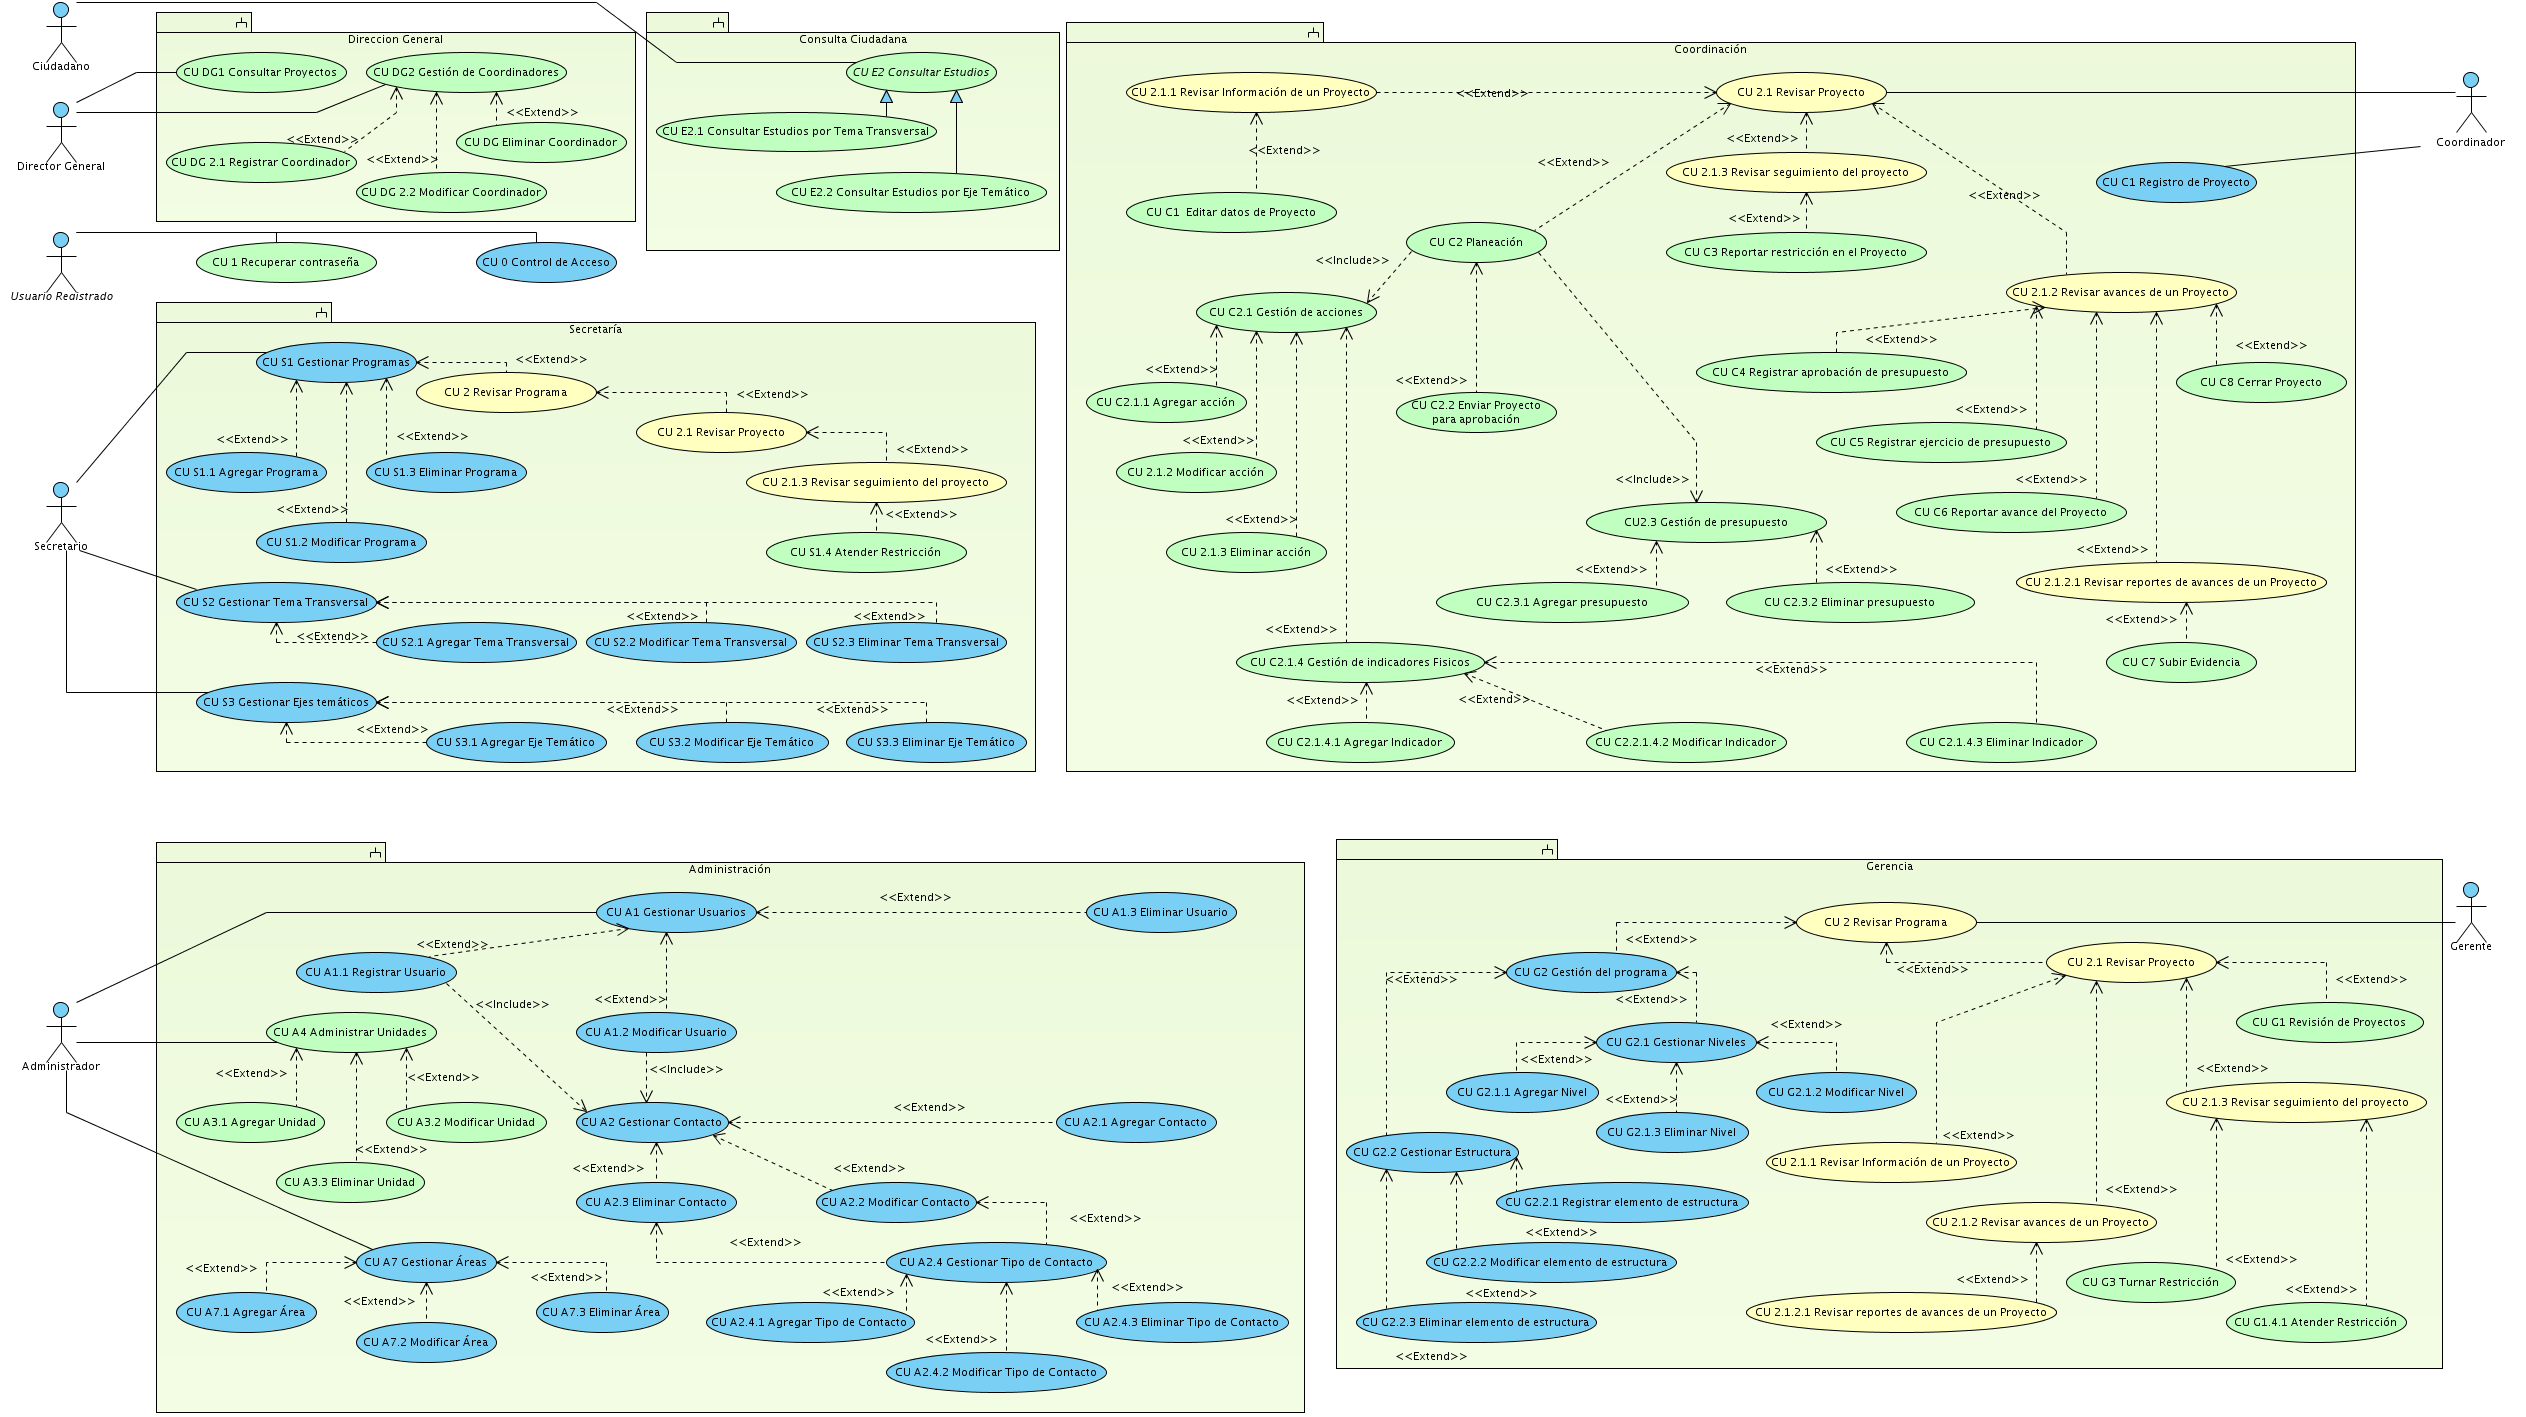
\includegraphics[angle=90,height=\textheight]{images/casosDeUso}
		\caption{Casos de uso del prototipo}
		\label{fig:default}
	\end{center}
\end{figure}

%=========================================================
\chapter{Modelo detallado del comportamiento, Control de acceso} 

%----------------------------------------------------------
\section{Diagrama de casos de uso}

\begin{figure}[htbp!]
	\begin{center}
		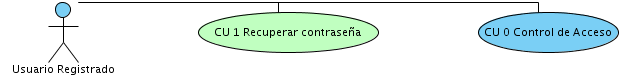
\includegraphics[width=.3\textwidth]{images/CUcontrolAcceso}
		\caption{Casos de uso para el control de acceso}
		\label{fig:default}
	\end{center}
\end{figure}

\cfinput{cu0iniciar_sesion/cu}

%=========================================================
\chapter{Modelo detallado del comportamiento, módulo de Ciudadano} 

%----------------------------------------------------------
\section{Diagrama de casos de uso}

\begin{figure}[htbp!]
	\begin{center}
		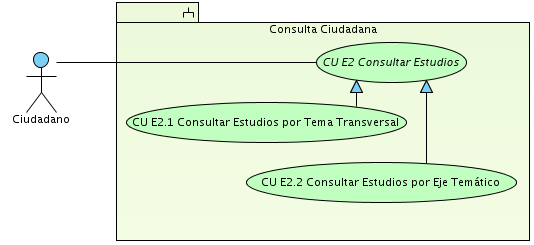
\includegraphics[width=.5\textwidth]{images/CUciudadano}
		\caption{Casos de uso del ciudadano}
		\label{fig:default}
	\end{center}
\end{figure}

\cfinput{cue2consulta_ciudadana/cu}

%=========================================================
\chapter{Modelo detallado del comportamiento, módulo general} 

%----------------------------------------------------------
\section{Diagrama de casos de uso}

\begin{figure}[htbp!]
	\begin{center}
		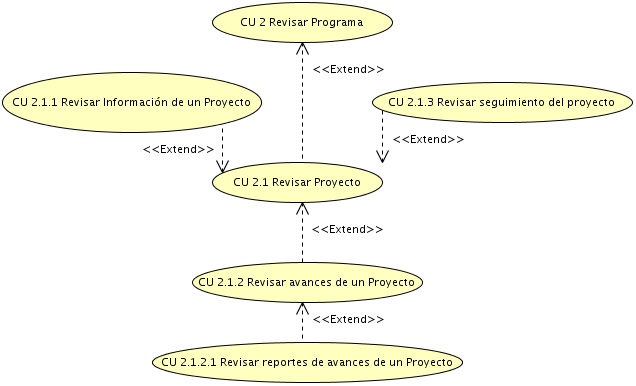
\includegraphics[width=.8\textwidth]{images/CU/general}
		\caption{Casos de uso generales}
		\label{fig:default}
	\end{center}
\end{figure}

\cfinput{cu2revisar_programa/cu}
\cfinput{cu2.1revisar_proyecto/cu}
\cfinput{cu2.1.1revisar_informacion_proyecto/cu}
\cfinput{cu2.1.2revisar_avances_proyecto/cu}
\cfinput{cu2.1.2.1revisar_reportes_avance_accion/cu}
\cfinput{cu2.1.3revisar_seguimiento_del_proyecto/cu}

%=========================================================
\chapter{Modelo detallado del comportamiento, módulo del Director} 

%----------------------------------------------------------
\section{Diagrama de casos de uso}

\begin{figure}[htbp!]
	\begin{center}
		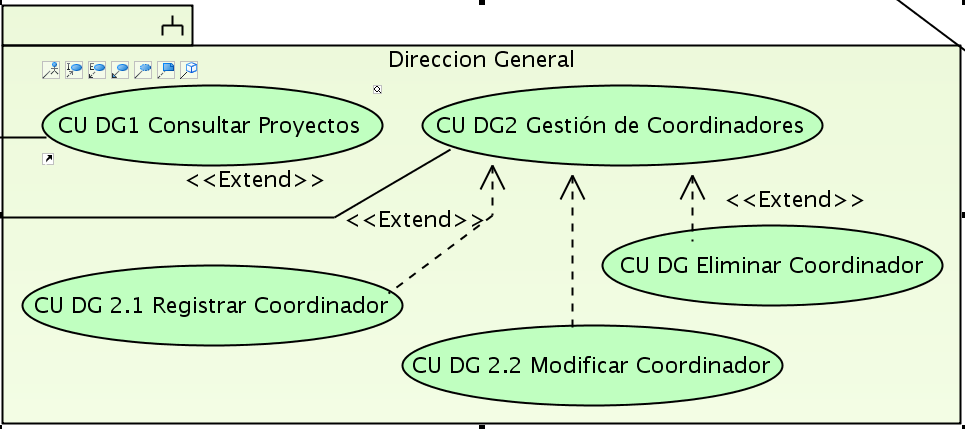
\includegraphics[width=\textwidth]{images/CU-DG}
		\caption{Casos de uso del Director General}
		\label{fig:default}
	\end{center}
\end{figure}

\cfinput{cudg1consultar_proyectos/cu}
\cfinput{cudg2gestion_coordinadores/cu}

%=========================================================
\chapter{Modelo detallado del comportamiento, módulo del Administrador} 

%----------------------------------------------------------
\section{Diagrama de casos de uso}

\begin{figure}[htbp!]
	\begin{center}
		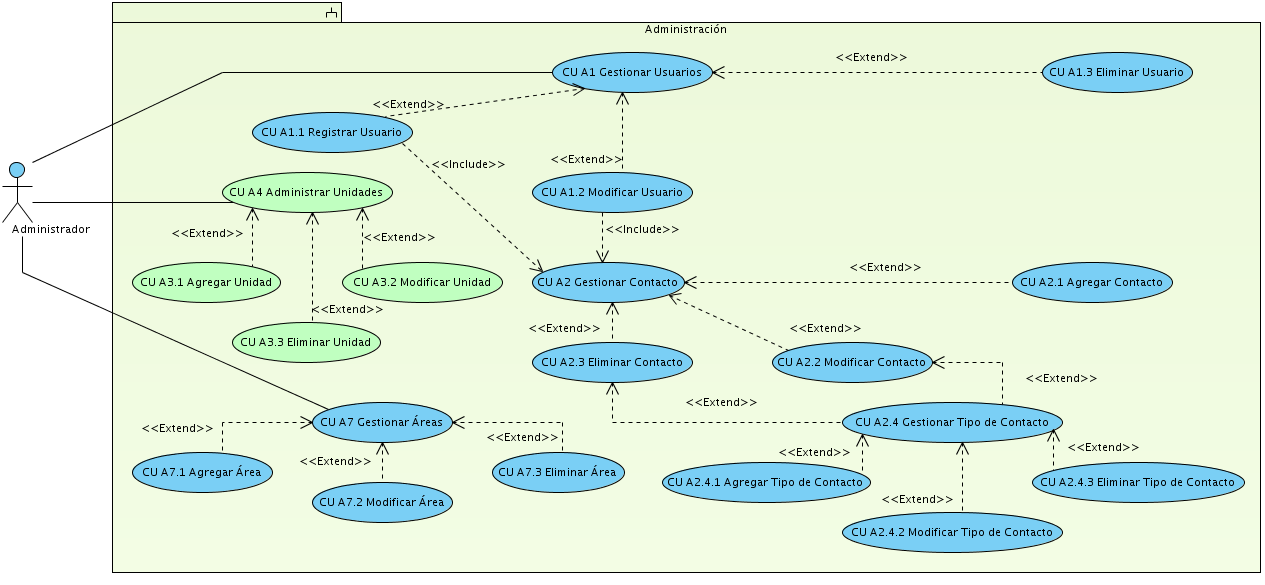
\includegraphics[width=\textwidth]{images/CUadministrador}
		\caption{Casos de uso del Administrador}
		\label{fig:default}
	\end{center}
\end{figure}

\cfinput{cua1usuario/cu}
\cfinput{cua2contacto/cu}
\cfinput{cua2.4tipo_contacto/cu}
\cfinput{cua4unidad/cu}
\cfinput{cua7area/cu}

%=========================================================
\chapter{Modelo detallado del comportamiento, módulo de Secretaría} 

%----------------------------------------------------------
\section{Diagrama de casos de uso}

\begin{figure}[htbp!]
	\begin{center}
		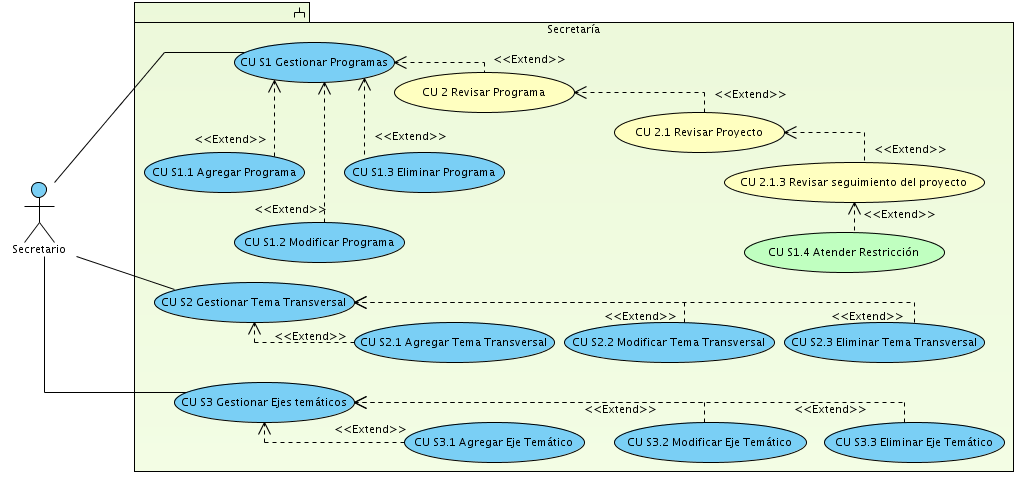
\includegraphics[width=\textwidth]{images/CUsecretaria}
		\caption{Casos de uso de Secretaría}
		\label{fig:default}
	\end{center}
\end{figure}


%----------------------------------------------------------
\cfinput{cus1programa1N/cu}
\cfinput{cus1.4atender_restriccion/cu}
\cfinput{cus2tema_transversal/cu}
\cfinput{cus3eje_tematico/cu}

%=========================================================
\chapter{Modelo detallado del comportamiento, módulo del Gerente} 
%----------------------------------------------------------
\section{Diagrama de casos de uso}

\begin{figure}[htbp!]
	\begin{center}
		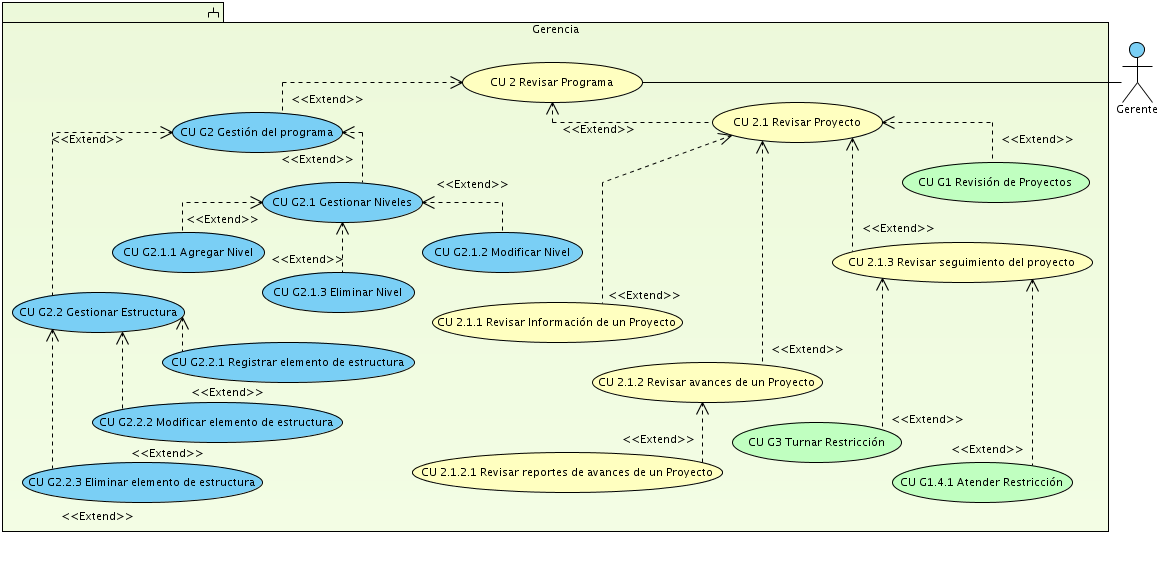
\includegraphics[width=\textwidth]{images/CUgerente}
		\caption{Casos de uso del Gerente}
		\label{fig:default}
	\end{center}
\end{figure}

\cfinput{cug1revision_de_proyecto/cu}
\cfinput{cug1.4.1atender_restriccion/cu}
\cfinput{cug2gestion_programa/cu}
\cfinput{cug2.1gestionar_niveles/cu}
\cfinput{cug3turnar_restriccion/cu}
%=========================================================

\chapter{Modelo detallado del comportamiento, módulo del Coordinador} 

%----------------------------------------------------------
\section{Diagrama de casos de uso}

\begin{figure}[htbp!]
	\begin{center}
		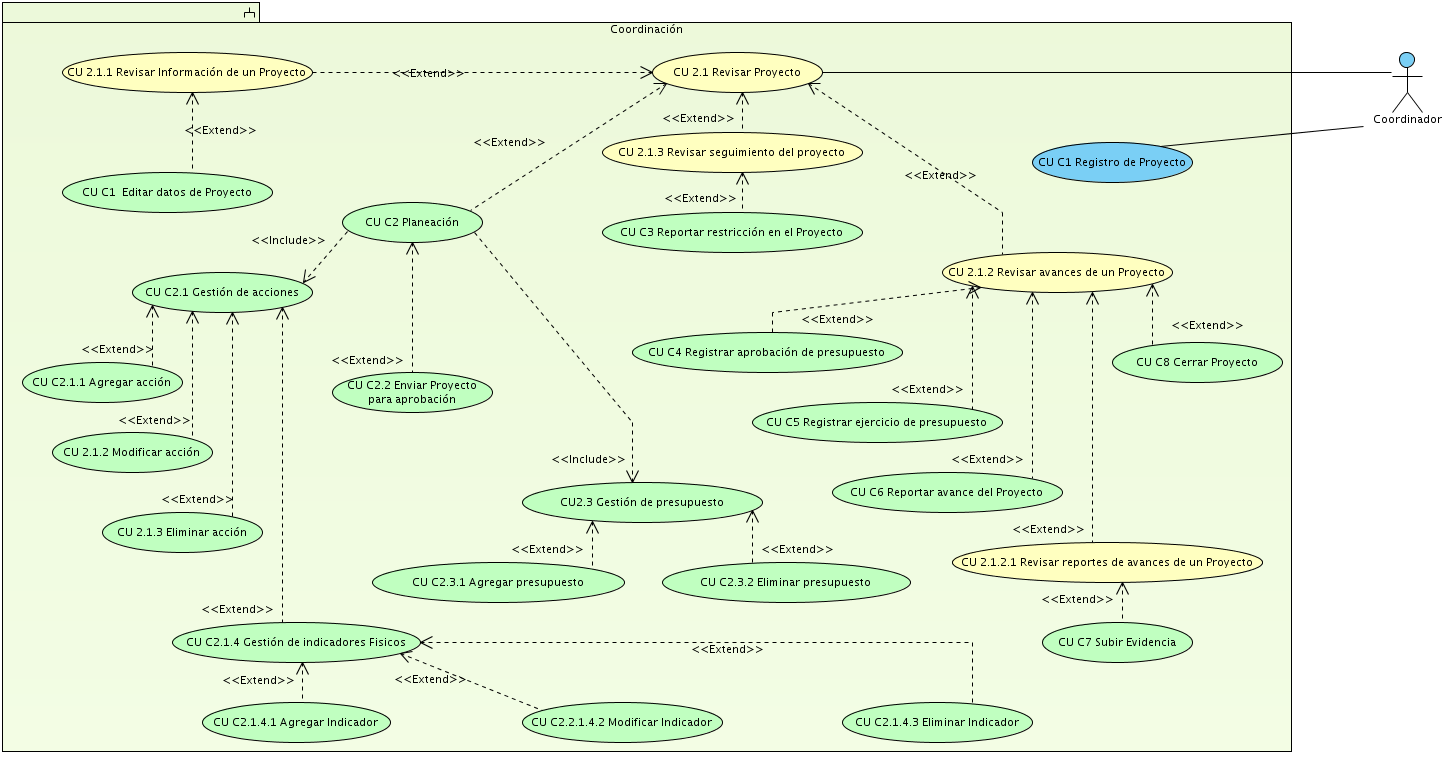
\includegraphics[width=\textwidth]{images/CUcoordinador}
		\caption{Casos de uso del Coordinador}
		\label{fig:default}
	\end{center}
\end{figure}

\cfinput{cuc1editar_datos_proyecto/cu}
\cfinput{cuc2planeacion/cu}
\cfinput{cuc2.2enviar_proyecto_para_aprobacion/cu}
\cfinput{cuc2.2.1acciones/cu}%Checar, en el diagrama dice que es cuc2 planeacion
\cfinput{cuc2.2.1.4indicadores/cu}%Checar, lo tengo en el diagrama como cu2.1.4
\cfinput{cuc2.2.2presupuesto/cu}%Checar,checar lo tengo como cu2.3.. que en si deberia ser cuc2.3
\cfinput{cuc3reportar_restriccion_en_el_proyecto/cu}
\cfinput{cuc4registrar_aprobacion_presupuesto/cu}
\cfinput{cuc5registrar_ejercicio_presupuesto/cu}
\cfinput{cuc6reportar_avance_proyecto/cu}
\cfinput{cuc7subir_evidencia/cu}
\cfinput{cuc8cerrar_proyecto/cu}
\cfinput{gestion_de_proyecto/estados}

%%=========================================================
\chapter{Modelo de interacción con el usuario, Control de acceso}
\section{Control de acceso}

\cfinput{cu0iniciar_sesion/IUIniciarSesion}
\cfinput{cu0iniciar_sesion/IURecuperarContrasena}

%----------------------------------------------------------

\chapter{Modelo de interacción con el usuario, módulo General}
\section{Generalidades}
\Instrucciones{ (notaciones, iconos, componentes comunes, etc.) }
\cfinput{generalidadesPantalla}

\section{Revisar Programa}
\cfinput{cu2revisar_programa/IUARevisarPrograma}

\section{Revisar Proyecto}
\cfinput{cu2.1revisar_proyecto/IURevisarProyecto}
\cfinput{cu2.1.1revisar_informacion_proyecto/IURevisarInformacionProyecto}
\cfinput{cu2.1.2revisar_avances_proyecto/IURevisarAvancesProyecto}
\cfinput{cu2.1.2.1revisar_reportes_avance_accion/IURevisarReportesAvance}
%\cfinput{cu2.1.3revisar_seguimiento_del_proyecto/}  Falta pantalla

%---------------------------------------------------------
\chapter{Modelo de interacción con el usuario, módulo del Director}
\section{Generalidades}

\Instrucciones{ (notaciones, iconos, componentes comunes, etc.) }
\cfinput{generalidadesPantalla}

\section {Gestion de Coordinadores}
\cfinput{cudg2gestion_coordinadores/IUAdministrar}
\cfinput{cudg2gestion_coordinadores/IUAgregar}
\cfinput{cudg2gestion_coordinadores/IUModificar}
\cfinput{cudg2gestion_coordinadores/IUEliminar}

\section{Consultar proyecto}
\cfinput{cudg1consultar_proyectos/IUConsultarProyecto}

%%=========================================================
\chapter{Modelo de interacción con el usuario, módulo del Administrador}

\section{Generalidades}
\Instrucciones{ (notaciones, iconos, componentes comunes, etc.)}
\cfinput{generalidadesPantalla}

%---------------------------------------------------------
\section{Gestión de Usuarios}

\cfinput{cua1usuario/IUGestUsuarios}
\cfinput{cua1usuario/IUAgregarUsuario}
\cfinput{cua1usuario/IUModificarUsuario}
\cfinput{cua1usuario/IUEliminarUsuario}
%\cfinput{cua1usuario/IUVisualizarUsuario}

%-------------------------------------------------------
\section{Gestión de Contactos}
\cfinput{cua2contacto/IUAdministrar}
\cfinput{cua2contacto/IUAgregar}
\cfinput{cua2contacto/IUModificar}
\cfinput{cua2contacto/IUEliminar}

\section{Gestión de Tipo de Contactos}
\cfinput{cua2.4tipo_contacto/IUAdministrar}
\cfinput{cua2.4tipo_contacto/IUAgregar}
\cfinput{cua2.4tipo_contacto/IUModificar}
\cfinput{cua2.4tipo_contacto/IUEliminar}

%-------------------------------------------------------
\section{Gestión de Unidades}

\cfinput{cua4unidad/IUAdministrar}
\cfinput{cua4unidad/IUAgregar}
\cfinput{cua4unidad/IUModificar}
\cfinput{cua4unidad/IUEliminar}

%-------------------------------------------------------
\section{Gestión de Áreas}
\cfinput{cua7area/IUAdministrar}
\cfinput{cua7area/IUAgregar}
\cfinput{cua7area/IUModificar}
\cfinput{cua7area/IUEliminar}

%%=========================================================
\chapter{Modelo de interacción con el usuario, módulo de la Secretaria}

%----------------------------------------------------------
\section{Generalidades}
\Instrucciones{ (notaciones, iconos, componentes comunes, etc.)}
\cfinput{generalidadesPantalla}

\section{Gestión de Programas}
\cfinput{cus1programa1N/IUAdministrar}
\cfinput{cus1programa1N/IUAgregar}
\cfinput{cus1programa1N/IUModificar}
\cfinput{cus1programa1N/IUEliminar}
\cfinput{cus1.4atender_restriccion/IUConsultaBitacoraSecretario}
%---------------------------------------------------------
\section{Gestión de Temas Transversales}
\cfinput{cus2tema_transversal/IUAdministrar}
\cfinput{cus2tema_transversal/IUAgregar}
\cfinput{cus2tema_transversal/IUModificar}
\cfinput{cus2tema_transversal/IUEliminar}

%---------------------------------------------------------
\section{Gestión de Ejes Temáticos}
\cfinput{cus3eje_tematico/IUAdministrar}
\cfinput{cus3eje_tematico/IUAgregar}
\cfinput{cus3eje_tematico/IUModificar}
\cfinput{cus3eje_tematico/IUEliminar}

%%=========================================================
\chapter{Modelo de interacción con el usuario, módulo del Gerente}

%----------------------------------------------------------
\section{Generalidades}
\Instrucciones{ (notaciones, iconos, componentes comunes, etc.)}
\cfinput{generalidadesPantalla}

\section{Gestion de Proyecto}
\cfinput{cug1revision_de_proyecto/IURevisionProyectos}
\cfinput{cug1.4.1atender_restriccion/IUConsultaBitacoraGerente}

\section{Gestion de Programa}
\cfinput{cug2gestion_programa/IUAdministrar}
\cfinput{cug2gestion_programa/IUAgregar}
\cfinput{cug2gestion_programa/IUModificar}

\section{Gestión de Niveles}
\cfinput{cug2.1gestionar_niveles/IUAdministrar}
\cfinput{cug2.1gestionar_niveles/IUAgregar}
\cfinput{cug2.1gestionar_niveles/IUModificar}
\cfinput{cug2.1gestionar_niveles/IUEliminar}

%\cfinput{cug3turnar_restriccion/} Falta pantalla

%%=========================================================
\chapter{Modelo de interacción con el usuario, módulo del Coordinador}
%----------------------------------------------------------
\section{Generalidades}
\Instrucciones{ (notaciones, iconos, componentes comunes, etc.)}
\cfinput{generalidadesPantalla}

\section{Planeación}
\cfinput{cuc2planeacion/IUPlaneacion}

\section{Gestión de Acciones}
\cfinput{cuc2.2.1acciones/IUAdministrar}
\cfinput{cuc2.2.1acciones/IUAgregar}
\cfinput{cuc2.2.1acciones/IUModificar}
\cfinput{cuc2.2.1acciones/IUEliminar}

\section{Gestión de Indicadores}
\cfinput{cuc2.2.1.4indicadores/IUAdministrar}
\cfinput{cuc2.2.1.4indicadores/IUAgregar}
\cfinput{cuc2.2.1.4indicadores/IUModificar}
\cfinput{cuc2.2.1.4indicadores/IUEliminar}


\section{Gestión de Proyecto}
\cfinput{cuc1editar_datos_proyecto/IUEditarDatosProyecto}
\cfinput{cuc2.2enviar_proyecto_para_aprobacion/IUEnviarProyectoAprobacion}
\cfinput{cuc2.2.2presupuesto/IUAdministrar}
\cfinput{cuc2.2.2presupuesto/IUAgregar}
\cfinput{cuc2.2.2presupuesto/IUEliminar}
\cfinput{cuc3reportar_restriccion_en_el_proyecto/IUConsultaBitacoraCoordinador}
\cfinput{cuc4registrar_aprobacion_presupuesto/IUAgregar}
\cfinput{cuc5registrar_ejercicio_presupuesto/IUAgregar}
\cfinput{cuc6reportar_avance_proyecto/IUAdministrar}
\cfinput{cuc7subir_evidencia/IUSubirEvidencia}

%%======================================================================

\chapter{Modelo de interacción con el usuario, módulo de Ciudadano}
%----------------------------------------------------------
\section{Generalidades}

\cfinput{generalidadesPantalla}
\section{Consultar Estudios}
\cfinput{cue2consulta_ciudadana/IUMenuCiudadano}
\cfinput{cue2consulta_ciudadana/IUConsultarEstudios}
\cfinput{cue2consulta_ciudadana/IUConsultarPorEje}
\cfinput{cue2consulta_ciudadana/IUConsultarPorTema}

%----------------------------------------------------------
\chapter{Catalogo de Mensajes} 
\cfinput{catalogoMensajes/mensajes}

%%======================================================================\chapter{Modelo del dominio del problema} 

\section{Diagrama Entidad/Relación}

  	\begin{figure}[h!]
 		\centering
 			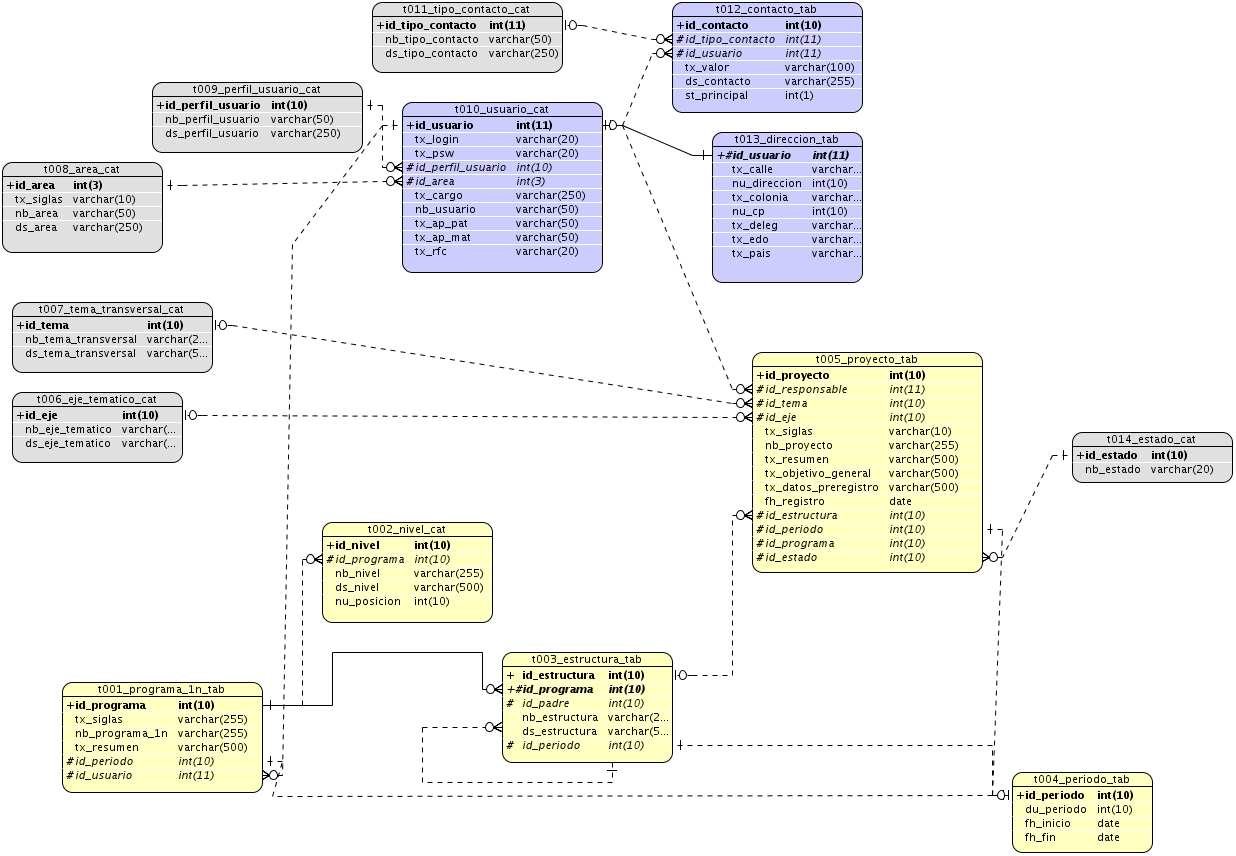
\includegraphics[width=.8\textwidth]{images/modeloER.jpg}
 		\caption{Unidad}
 	\end{figure}

\section{Diccionario de Datos}

\cfinput{diccionario}



\end{document}
